\chapter{Positioning the Thesis}
\label{chapter:positioning}

Master's theses don't live in a vacuum. To position the thesis and provide the
best possible outcome for Aalto University we have made an effort to find out what
is the current state of research data management, publishing and sharing as well as what
are the current challenges and projects in the Finnish landscape. While the
literature review in Section \ref{chapter:background} covered the overall view
of the current status of publishing and sharing research data and research
papers, the goal of this thesis is to provide practical value towards implementing
research data management, publication and sharing systems. Practical
insights lie within people working in the area.
The tools used to position the thesis were interviews, benchmarking existing
solutions and a questionnaires.

\section{Researcher interviews}
\label{sec:expert_interviews}

Scientists and researchers are the core user group of any publishing or sharing
system since they are the ones generating the data to the system and possibly populating
the system. The research also shows that a successful repository system requires
user engagement \cite{DBLP:conf/ercimdl/Martinez-UribeM09}. Scientist and
researcher interviews were conducted within different research groups and
researcher in Aalto Otaniemi campus. The goal of these interviews was to learn
how data management is taught and used in Aalto University and what are the
scientist and researchers perceptions on sharing and publishing research data.
Previous experiences with sharing and using others' data were also gathered.

The interviews presented here were conducted in the beginning phase of this
thesis - later, more in depth interviews were conducted to test a possible
solution. This discussion can be found in Section \ref{chapter:prototype}.

In an interview with a research group\footnote{M. Nurmela and the Complex
Networks group at Aalto University (\url{http://becs.aalto.fi/en/research/complex\_networks}),
personal communication, July 31st, 2015} the findings fell in line with the
findings from literature. As of writing of this thesis, data management is not
systematically taught for the researchers and
there is no culture or experience in data sharing. Upon questioning it became
clear that the data in the possession of the researchers would have required
a lot of cleaning and metadata additions prior to publishing - this is no surprise
considering the fact that the datasets they were using were not designed to
go public in the first place. Though lack of metadata practices and lack of
publishing infrastructure were also brought up.

Some members of the research group had shared some of their datasets through
public cloud services such as Google Drive\footnote{\url{http://drive.google.com/}}
with collaborators and used others' datasets. This also raised the point that
in order to use others' datasets they had been asked to cite the papers that
used that dataset, underlining the the undeveloped culture of research data
sharing. Some members of the group saw big advantages in making research output
public, especially from the angle of reproducibility, but also raised concerns
about the privacy issues that for example telecommunication data would cause.
The members of the group were also concerned about about the size of their
data, since using the existing solutions to share hundreds of gigabytes worth
of data would prove cumbersome.

One member of the group had taken a role of a mentor with the data management
issues, teaching the others to use databases and version control software to
handle their data and code. The other members of the group, interviewed
separately, noted that an effort had been made towards better policies in data
handling. The group pointed out that personalized assistance and word of mouth
were an efficient way to learn ''boring'' things like data management. Own
previous experience and learning by doing seemed to be the main way people had
learned to, for example, comment their code or arrange their research data into
databases so that accessing them would require less time and managing code
would be easier.

Discussions with the complex networks groups also brought up the point that
even though some data could be published for all the world to see, some data
should be only accessible to people within Aalto University and some should
even have a more fine grained access control set to them.

In a separate interview with a brain image researcher\footnote{M. Nurmela and
E. Glerean, personal communication, August 13th, 2015} similar concerns arose.
Brain imaging data is large and that makes sharing it hard. Brain images are
also considered personal data and publishing them is problematic. The
researcher expressed interest in sharing and using others' datasets, but
lacked the tools to do so.

\iffalse
\section{Scientists}

Scientists would be the main user or stakeholder that would use the system. It
is important that a system that would help them store and publish research data
would provide value for them without being another system that is a huge
annoyance to use.

\subsection{The goal of the interviews}

It is interesting as to what is the current status of research data management
and how research data is being published. Also what was learned in interviews 
with other stakeholders it became clear that research data management covers
much more than just the publishing part, so it was important to find out
whether the scientists were actually being trained to handle research data.

The secondary goal is also to gain input on how the system to manage and
publish research data should look like if it were to be implemented.

\subsection{Results of the interviews}

\fi

\section{Science IT staff}
\label{sec:sci_it}

If a system to publish and share research data would come to be it would have
to be maintained and run by people other than the researchers, since the job of
the researchers is to do research and not to maintain software systems. With this
in mind the people managing the scientific IT systems are a key component to
building a successful research data management, publication and sharing
platform.

In interviews with a scientific IT systems specialist\footnote{M. Nurmela and
M. Hakala, personal communication, July 1st and 7th, 2015} the findings again
aligned with the findings from literature. There is a lack of metadata
standards that would make data storage and management uniform across
institutions and disciplines. Finland has projects going on related to open
science\footnote{\url{http://avointiede.fi/}} and CSC\footnote{\url{https://www.csc.fi/}} is
building scientific computing environments for Finnish institutions (research,
library, archival, education and such). According to the specialist
collaborating with all these ongoing projects would benefit both parties and
also allow Alto University to develop systems that are not just point
solutions. This would also make sense from a financial point and practical
point of view, since research is nowadays done in collaboration with other
institutions and working together would enable that.

From the point of view of IT system specialist the ideal system for research
data includes the whole lifecycle of the data. This entails education on how
to manage the data from the creation to the publishing and infrastructure that
can be tailored to fit the different user needs. Research data is comes in
many forms so a solution that is not flexible would be unsuitable.

University of Jyväskylä has implemented a Dataverse data repository 
system\footnote{\url{https://dvn.jyu.fi/dvn/}}
as well as an iRODS\footnote{\url{http://irods.org/}} system to manage and
store research data. In an interview\footnote{M. Nurmela, I. Korhonen and A.
Auer, personal communication, August 19th, 2015} they noted that nowadays
universities need a platform to publish research data. Jyväskylä is among the
first in Finland to implement a data policy in practice, offering an
infrastructure to manage data during the research projects and publish the
results in the end (even though Dataverse and iRODS are not currently
easily compatible with each other, though some work has been done for
that\footnote{\url{https://irods.org/wp-content/uploads/2014/06/Odum-DFC-iRODS-Boston.pdf}}).

The Jyväskylä experts told that while the Dataverse system was easy to install
and modify to accept Jyväskylä University credentials, it still had a long way to go
before it was universally accepted within the university. At the time of
writing this, the Jyväskylä Dataverse has been running for approximately a
year and it contains a very small amount of datasets. Some research groups,
however, are using it manage their internal datasets. As to how to get the
more datasets into the system, they planned to continue educating about it
and making it that way a part of researchers' routine.

As of writing of this thesis Jyväskylä is more involved in development of the iRODS system, having
developed a system called Kanki to facilitate collaboration between researchers
\cite{irodsinproceedings}. The Kanki system is a desktop interface to the iRODS
system that allows users to easily access and modify data stored in the iRODS
data grid. The Kanki system is not about publishing research data but data
management during a research project. iRODS also has federation capabilities,
meaning that two iRODS instances could be integrated such that you could
access the data from the other system. When writing this Jyväskylä and CSC
were planning to start testing the federation capabilities. Following up on that
on a later date would be interesting.

\iffalse
If there was to be a system to manage and publish research data, it would have
to be maintained by someone. The obvious answer is to go to the administrators
of institutional software infrastructure.

\subsection{The goal of the interviews}

What is the stance of the administrative side on a data repository? How does it
fit the role of the infrastructure administrators? Building software systems is
not only about what people want and what existing systems prove to be the best,
human factors and elements like funding affect these decisions.

At least in Aalto the staff maintaining the infrastructure are also aware about
who are the people hosting research data on school infrastructure, making them
also knowledgeable on how things are handled right now.

\subsection{Results of the interviews}

\fi

\section{Project managers on research data related systems}

Building and running software systems requires commitment not only from the
primary users discussed in Sections \ref{sec:expert_interviews} and
\ref{sec:sci_it} but the management that supports them. The priorities of the
managerial types might not lie in the usability or maintainability of the
system, but rather in managing costs and minimizing risks.

Interviewing a manager from Aalto side it was made clear that there is a
desire to minimize the systems we have to build and
maintain ourselves - since CSC exists to provide scientific computing and
storage resources, why should we not use them? Non established or new fields
of science could have value from a local repository, but those that have
international or discipline specific repositories could use those as well.\footnote{M. Nurmela, A. Sunikka, personal communication, July 17th, 2015}
Managing research data is seen as a problem and a consensus best solution has not
emerged.

The Finnish National library is in charge of long term preservation of relevant
objects in the Finnish research. They are building a long term storage
solution\footnote{\url{http://avointiede.fi/tutkimus-pas}}, data management
plan tool\footnote{\sloppy\url{http://portti.avointiede.fi/tutkimusdata/tuuli-tyokalu-tutkimuksen-datanhallinnan-suunnitteluun}} and managing the Finnish unique identifier
service\footnote{\url{http://www.kansalliskirjasto.fi/fi/julkaisuala/urn.html}}.
They also manage a Finnish cultural repository\footnote{\url{https://www.finna.fi/}}.

The most important thing to for the project manager at the National Library
was that metadata associated with the data has to be good - otherwise
archival, management and reuse is impossible. Making metadata work within an
institution requires commitment from all levels of management and tools to
facilitate that. It is also important to note that even if two systems within
different organizations would be technologically perfectly compatible,
the bottlenecks might stem from different policies in different organizations
and the bureaucracy that comes with it. This thought lessens the burden for all
technology to be perfectly compatible.\footnote{M. Nurmela and E. Keskitalo, personal communication, August 21st, 2015}

\iffalse
Implementation and running of different systems related to research data
management and publishing are being implemented and developed around Finnish
institutions. While people working on and with these systems were included in
the previous two sections (backwards reference) there are people who are in
charge of those systems and make the decisions on which to purchase.

\subsection{The goal of the interviews}

Systems that have to do with entities as big as universities or even nations
need management and getting a view from only the people using them is not
sufficient when designing such a system. People in managerial positions have
different objectives and needs for a system like this.

From people in positions like this it is important to learn about the bigger
picture. When dealing with a concept like sharing research data it makes sense
to try make systems talk to each other and not everyone to implement their own
system in their own silo.

\subsection{Results of the interviews}

\fi

\section{Librarians}

Publishing research data requires expertise in digital publishing and metadata creation
experience. University libraries are experienced in publishing digital research
papers (open access or restricted access) and making metadata descriptions
about digital and physical publications. This makes librarians and libraries
and essential part in bringing research data to the open publishing world.

In an interview with the people responsible of the digital publishing at Aalto
University Library\footnote{M. Nurmela and A. Rousi, personal
communication, September 30th, 2015} the essential role of
librarians as the classifiers and describers of the data was brought up. Professional data
handlers can do very good metadata descriptions, even if they are missing
some of the domain knowledge related to the research data. The librarians
also handle the relationships to the publishers - though what is the role
of traditional scientific publishing authorities in the future when organizations
can publish datasets and even research papers papers easily on their own remains
an open question.

Aalto University library runs the Aaltodoc service\footnote{\url{https://aaltodoc.aalto.fi/}}
which contains full text materials on research papers and theses published
in Aalto University. The system runs on on DSpace\footnote{\url{http://www.dspace.org/}},
an institutional repository software for publishing digital objects. DSpace
focuses on publishing research papers, but the person in charge of the system
reckoned that it probably could be modified to host small datasets as well.
This would require some additional work of course, so a better way could be to
link the research papers the relevant datasets in the corresponding systems.\footnote{M.
Nurmela and J. Nevala, personal communication, August 27th, 2015}

The National Library of Finland is in charge of implementing long term storage
and archival of important datasets and other research material. From that point
of view and also research data in general the biggest challenges are not
technical - software systems to store data and manage it exist, but making it
so that institutions themselves commit to managing and storing data is the
bigger challenge. And once different institutions are able to manage their own
data, the collaboration between the institutions' systems is likely to be
more difficult in the policy and bureaucracy sense. There are also many
unresolved questions related to long term storage. Who decides what datasets
are used for the long term storage? What kind of metadata long term storage
requires in addition to the metadata already in the original dataset? What
is the most suitable file format for long term storage, since tools and
software used to create it outdated relatively soon? The work
to figure out these things and the Finnish long term archival project is going
on during the writing of this thesis.\footnote{\label{keskitalo}M. Nurmela and E. Keskitalo, personal communication, August 21st, 2015}

From curation point of view persistent identifiers are very important for
all kinds of research outputs. Since research data publishing is a new
phenomenon, it's still undecided what kind of identifier should be used
with it.\footnotemark[\getrefnumber{keskitalo}]

The universities already have datasets stored within their systems and one
challenge would be to get these datasets public as well. Manual work on that
would be futile, which is why a system that would extract the existing data
from unversities' systems automatically would be useful.\footnote{M. Nurmela
and J. Kesäniemi, personal communication, September 2nd, 2015}

\iffalse
Librarians are metadata experts. They are trained to describe scientific
content, manage and sort that content and nowadays they also work with digital
publishing. In some libraries across the globe (citation) the libraries have
taken responsibility of also publishing research data.

\subsection{The goal of the interviews}

What is the current status of digital publishing in Finland? And how do the
libraries themselves see their role when publishing research data enters the
equation. How should we organize the collaboration between libraries and
scientists?

\subsection{Results of the interviews}

\fi

\section{Course organizers}

In addition to research, the mission of universities is to teach. With the
world of research moving to the direction of more and more data intensive science
there is a need universities need to adapt and offer students the possibility to study with
relevant datasets. Aalto University has started offering a minor in Data
Science in order to cater to this need.\footnote{\url{http://studyguides.aalto.fi/minors-guide/2015/en/sci/sci-minors-for-all-aalto-students/analytics-and-data-science.html}}.

In an interview with the people in charge of the Aalto Data Science minor
it became clear that even though data intensive science is taught, there is no
Aalto infrastructure for the teaching. Datasets and the computing power are
acquired from vendors which had caused some awkward arrangements since the
access to the outside resources had to be controlled more tightly than just
on Aalto level. These issues can be worked out though and from the point of
teaching it would be nice to have data available from within the university,
data and computing resources could also be acquired elsewhere.\footnote{M. Nurmela,
J. Bragge and P. Malo, personal communication, August 6th, 2015}

The people in charge of teaching also could offer insight to the question about
the basic skills that go to data analysis. The question is interesting since
in order to leverage the fact that science is becoming more and more data
intensive scientists need to possess skills both to analyze their data and
manage it in a sufficient way. The skillset that's required for data handling
and management is largely programming, since naturally the analysis is
computerized and things such as cleaning and preparing data for analysis is
most efficient when done programmatically. On the other hand, the data analysis
part asks for skills in algorithmics and statistics. When we take into account
that the Aalto Data Science minor, for example, is open for students from all
fields of science, it seems that we need to be teaching a new set of skills to
almost all students that want to take part into the new wave of data intensive
science.

\iffalse

Teaching is another role within the university that would benefit from the fact
that research data would be readily available for the students to consume and
run analysis on. If we wanted to make research data management an integral part
of scientists' daily routine it would have to be integrated to the teaching
regime taught in schools.

\subsection{The goal of the interviews}

Aalto University has a minor in Data Science, but does it have any means to
support that? How is data science and in its wake data management taught
currently in the university?

\subsection{Results of the interviews}

\fi

\section{CSC}
\label{sec:csc}

CSC is the national computing service provider for Finnish institutions. They
offer both computing power and disk space for Finnish institutions and they
are a state-owned non-profit organization.\footnote{\url{https://www.csc.fi/csc}}
Their role is interesting when it comes to research data management and
publishing, since they already offer computing services to the relevant
institutions in Finland. After all, one goal of publishing and sharing
research data is to enable collaboration and involving the one institution
in Finland that offers services to all the other institutions makes sense in
that regard.

One of CSC's services related to research data management is the IDA
service\footnote{\url{http://avointiede.fi/ida}} that is specifically
designed to store research data and the related metadata. CSC also maintains
Etsin\footnote{\url{https://etsin.avointiede.fi/}}, a service to host
metadata related to research data as well as links to the location of the data.
Etsin itself does not contain datasets.
These efforts fall under the national project of Open
Science\footnote{\url{http://openscience.fi/}} (Avoin Tiede ja Tutkimus in
Finnish) that promotes the openness of research and science. On the top level
these initiatives have been put into motion by the Ministry of Education and
Culture\footnote{\url{http://www.minedu.fi/OPM/?lang=en}}.

The IDA service, however, has not been very widely adopted as a place to store
and share research data. This has to do with IDA's user interface and the fact
that the iRODS backend is not designed for publishing information. Issues with
policies and permissions also hinder the publication process.\footnote{M.
Nurmela and S. Westman, personal communication, August 14th, 2015} In addition
to the technical matters there is of course the fact that institutions, such as
universities, do not have a very well developed culture for research data
management or publishing which also contributes to this.

CSC also implements a service called AVAA\footnote{\url{http://avaa.tdata.fi/en/}},
which contains spatial datasets such as open street maps for Finland and data from
weather stations around Finland. It seems that it is not designed for all kinds
of datasets or it has not been adopted for other uses.

\iffalse
CSC offers an interesting angle to the research data management problem. CSC
offers nationwide computing services and they should have a role in sharing and
managing research data.

\subsection{The goal of the interviews}

CSC must have some plans and current ideas on how to manage and share research
data since the world is moving towards publishing research data. It also makes
sense from their point of view to offer both computing power and storage
services and it would be interesting to know what are their plans in that
sector and if they do not have plans what is going on with that.

\subsection{Results of the interviews}

\begin{itemize}
    \item many experts
        \begin{itemize}
            \item scientists
            \item science IT staff
            \item people in charge of policies and development of university
                  systems
            \item developers in libraries
            \item library representatives
            \item project managers at CSC (in charge of nationwide computing
                  services)
        \end{itemize}
        \item fill in input from each once it's time to write those
        \item notable common findings
        \begin{itemize}
            \item metadata management is a huge problem
         demand to publish research data   \item no education, tools or any idea on how to work with that
            \item no experience in data sharing
            \item not willing to use lots of time for metadata management
            \item the university would prefer not to store their own
                  datasets, but would rather work with other places
            \item library should have a role in managing metadata and coaching
                  the scientist with their dataset management
            \item data intensive science is being taught in Aalto, but without
                  own infrastructure
        \end{itemize}
        \item also a common conclusion here is that there is not consensus
              within Finland on how to arrange ourselves with research data
        \item there is the nationwide computing service provider, CSC, but
              there is no common push towards data repository or managing
              research data
\end{itemize}

\fi

\section{Research data management questionnaires}
\label{sec:questionnaire}

Separately from this this thesis wo studies were conducted in Aalto University about research data management
and sharing. The goal of the studies was to find out the current needs as well
as the current status of research data management within Aalto University. The
studies were carried out as questionnaires and the questionnaires were
distributed to all branches of Aalto.

The first questionnaire \cite{survey1} divided
the research process in the context of research data into four phases, which
are the defining of the research scope, the research, publishing the research
data and archiving the research data. 87 people submitted answers to the study from all the
schools in Aalto. The breakdown respondents is shown in Figure \ref{fig:chart_answers}.

\begin{figure}
    \begin{centering}
        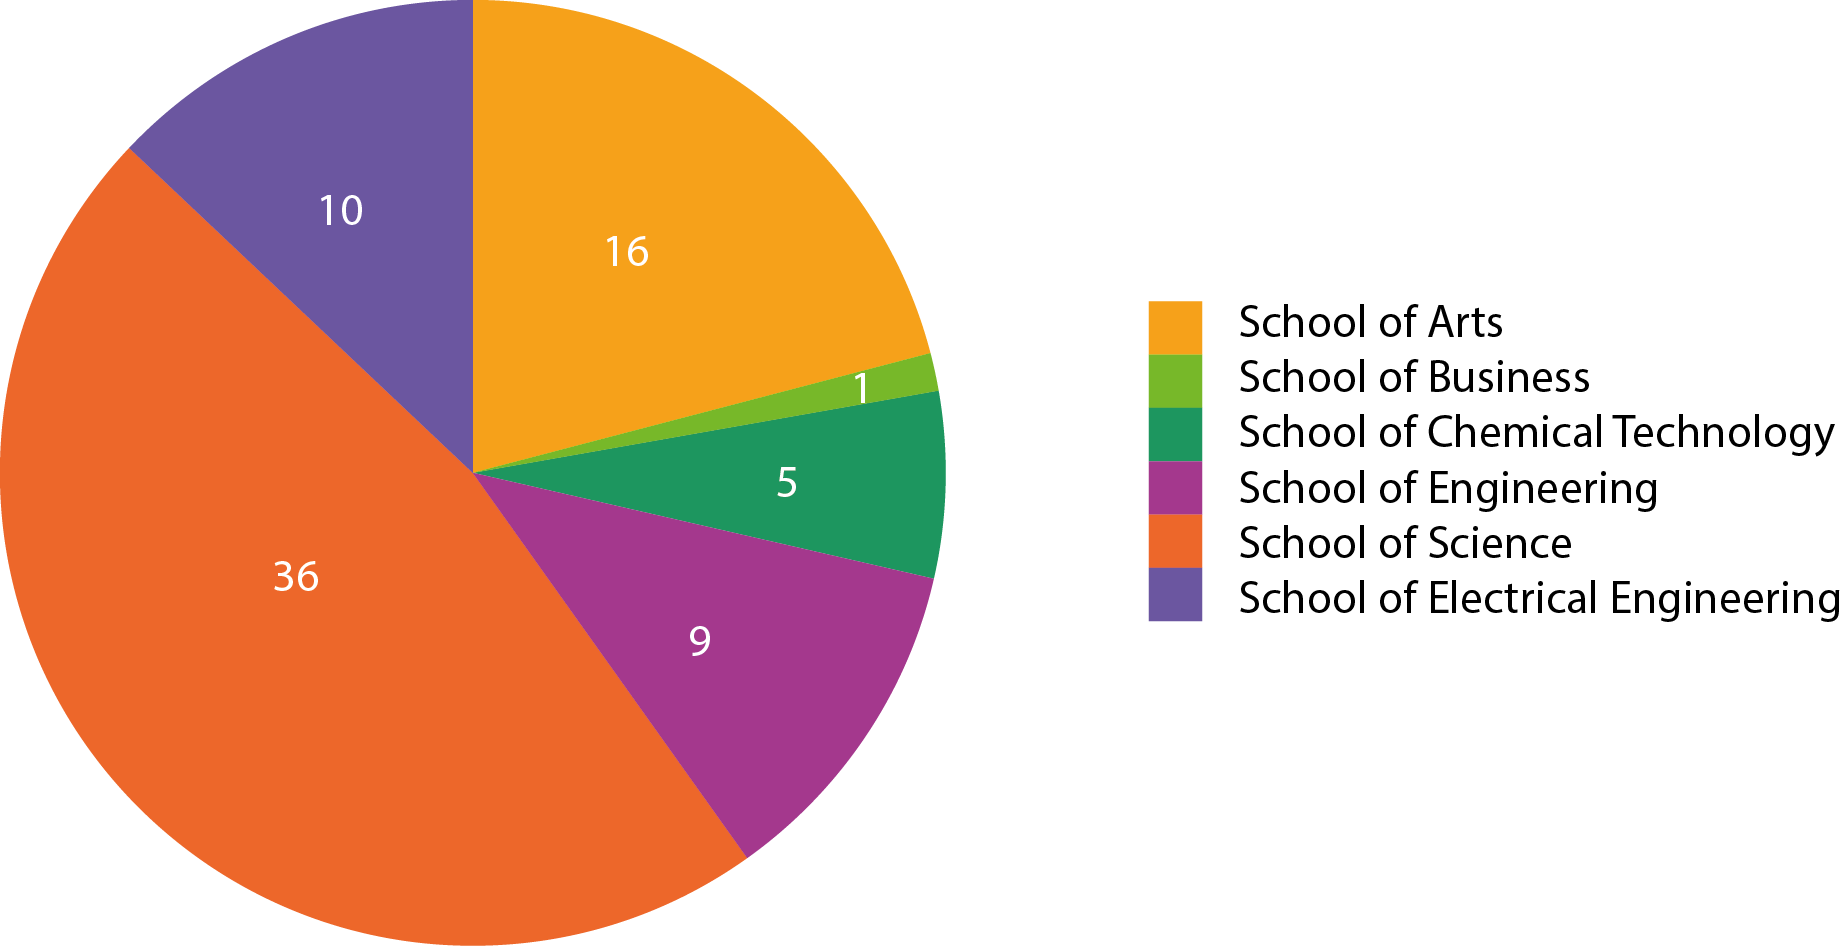
\includegraphics[width=\textwidth]{images/chart_answers2}
    \end{centering}
    \caption{The respondents to the first questionnaire, divided by the school of the respondents}
    \label{fig:chart_answers}
\end{figure}

The biggest challenges reported by the questionnaire were with the actual
research process and the archiving of data, as outlined by Figure
\ref{fig:challenges}. During the scope defining phase of the research the
research data challenges mentioned were storage, availability and version
control. The actual research phase contained many challenges, biggest of which
were the lack of storage space, the size and amount of files generated (the
current system could not handle them) and the challenges with data
availability. The problems with sharing research data came from the lack of
sharing infrastructure, version control, storage space (quantity and
persistence - no way to persist digital files) and other restrictions, such
as privacy concerns or classified data. The single biggest problem with
archiving research data was that there is no infrastructure for archiving
research data.

\begin{figure}
    \begin{centering}
        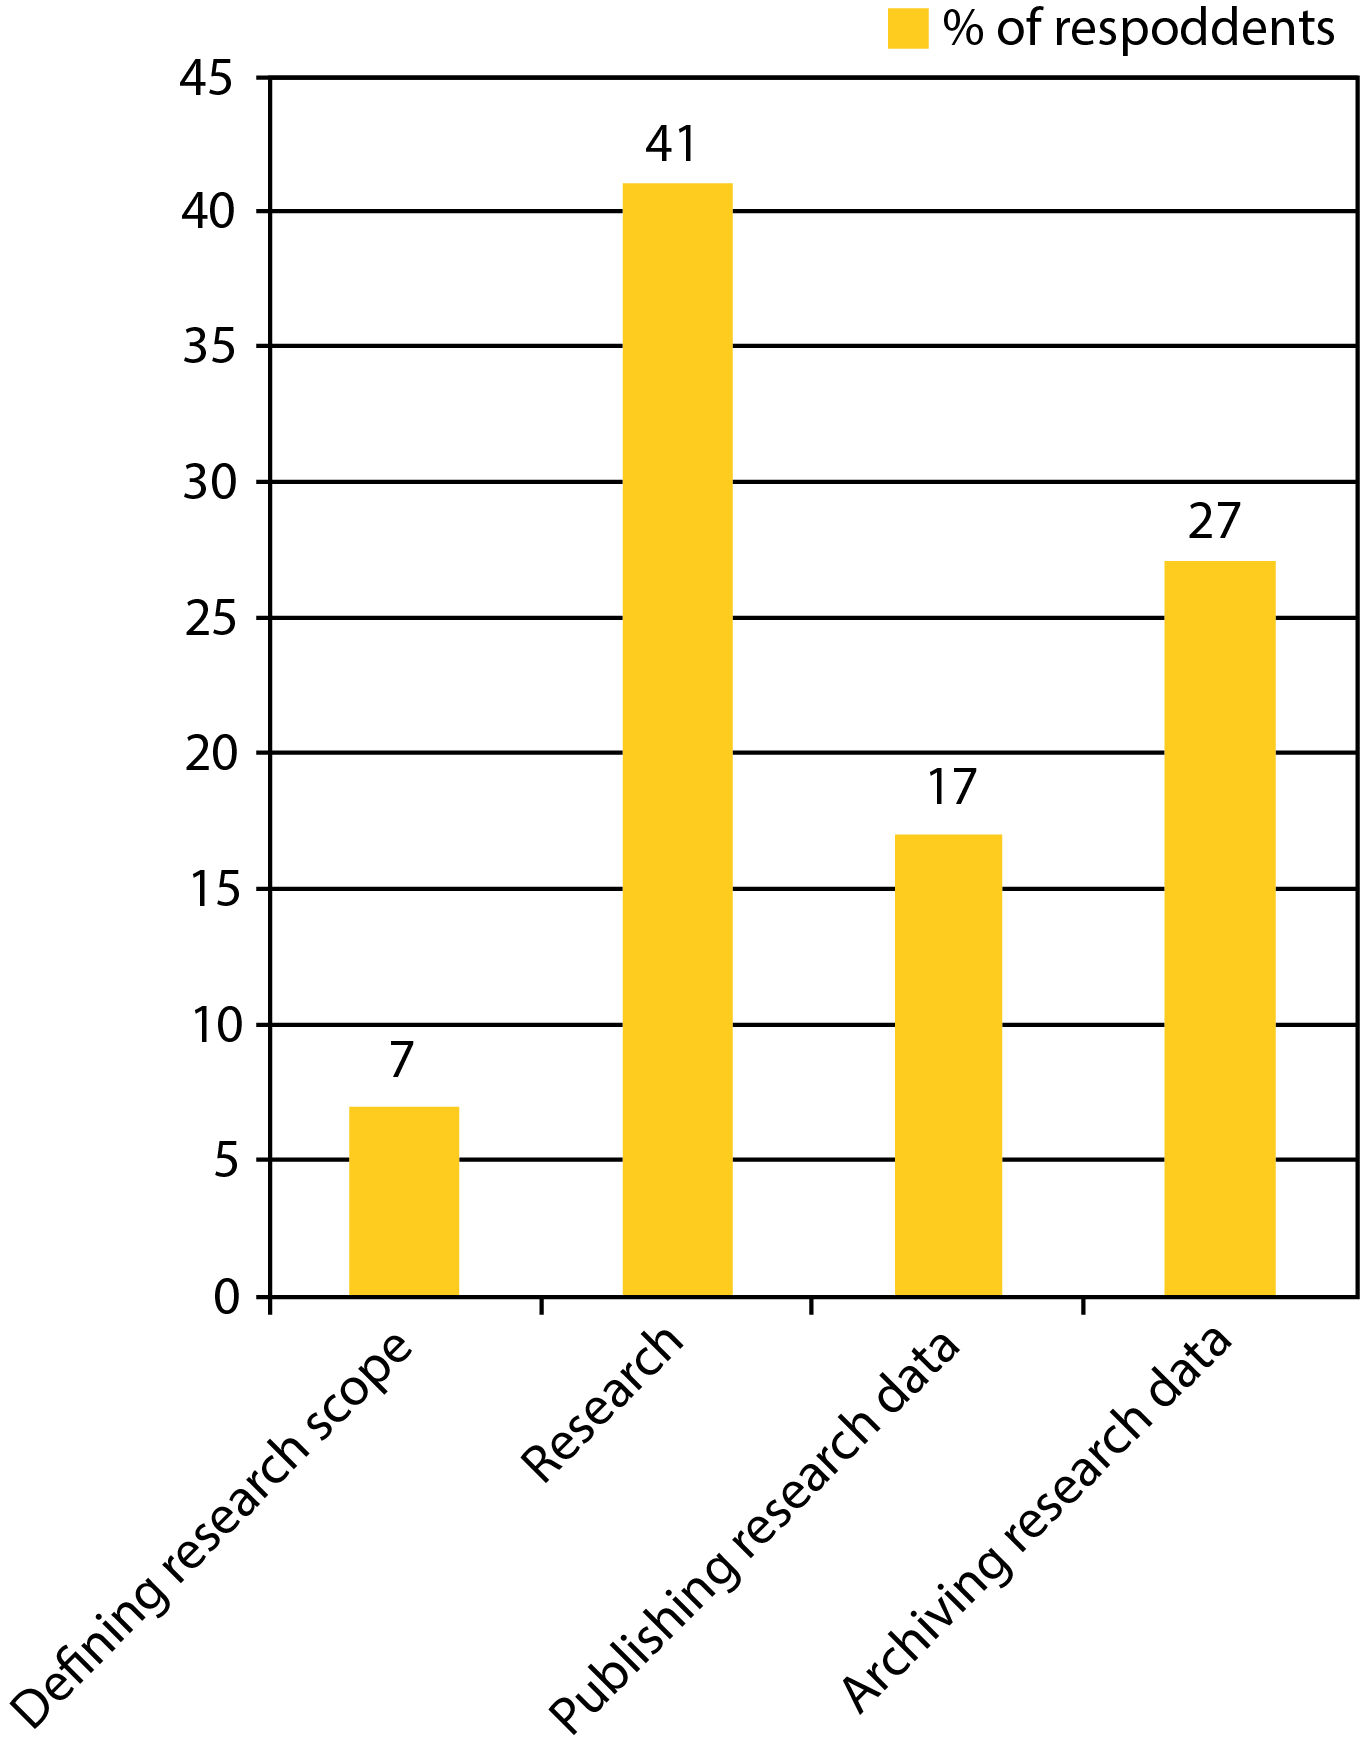
\includegraphics[width=\textwidth]{images/challenges2}
    \end{centering}
    \caption{Where the biggest challenges lie with research data management, divided by the phase of research process}
    \label{fig:challenges}
\end{figure}

\pagebreak

The greatest need for services derived from the first questionnaire was
reported in storing data, metadata, finding data, archiving, sharing
and backing up data. The challenges where the requirements span from are both
technological and policy related. In the list below the the answers are
compiled by percentages:

\begin{itemize}
    \item The name of the folder/file or the location of the folder/file is
          forgotten or poorly described, approx. 35\%.
    \item Ownership of the data, approx. 30\%.
    \item Not enough disk space, approx. 30\%.
    \item Version control, approx. 30\%.
    \item Non functional or corrupted equipment, 29\%.
    \item Sharing data with partners and collaborators, 24\%.
    \item Unwanted deletion of data, 22\%.
    \item Complicated user interface, approx. 20\%.
    \item Forgetting password, 17\%.
    \item Access rights, approx. 12\%.
    \item Failed backup, 8\%.
\end{itemize}

The second questionnaire \cite{survey2} has 368 respondents, divided into different branches
of Aalto as shown in Figure \ref{fig:answers_branches}.


\begin{figure}
    \begin{centering}
        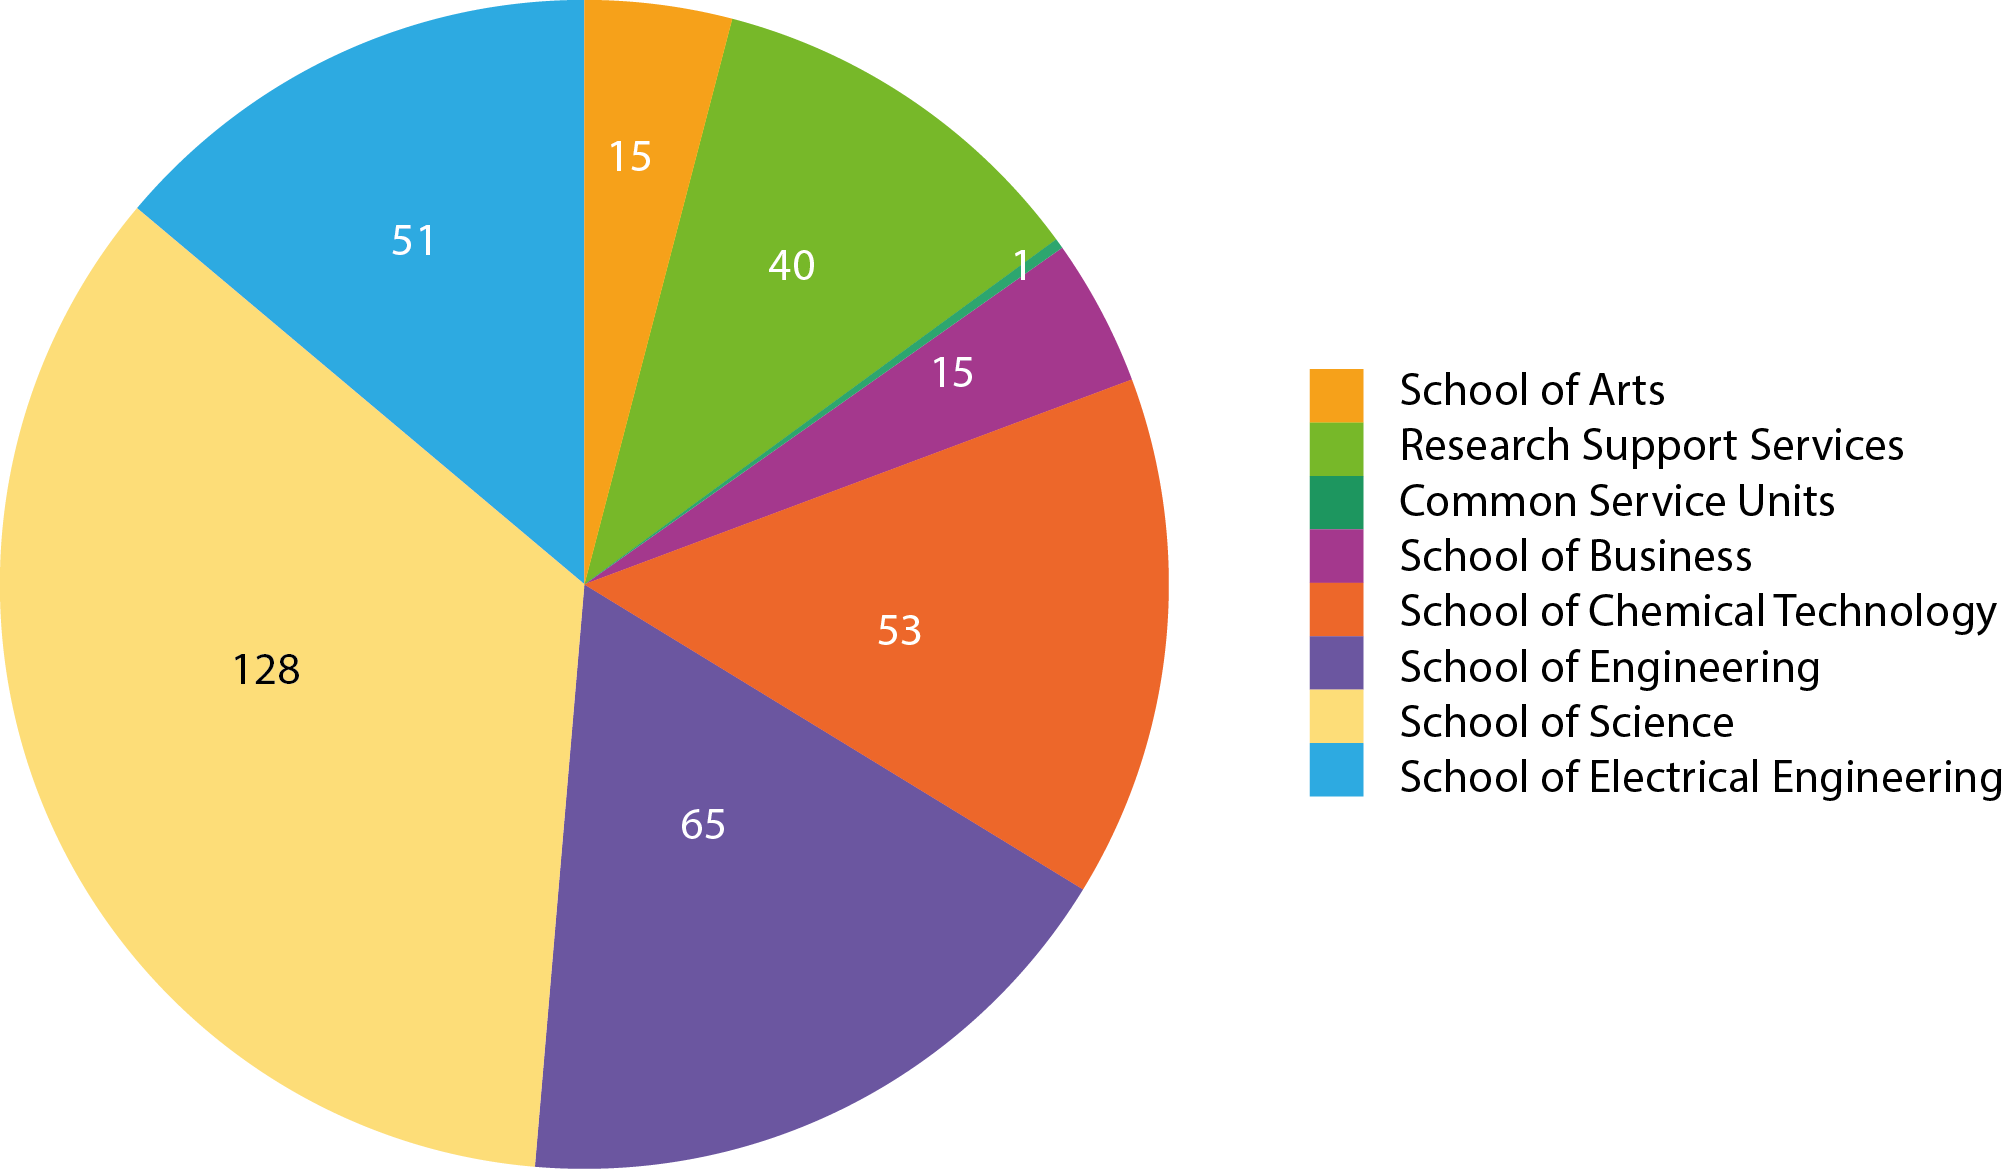
\includegraphics[width=\textwidth]{images/answers_branches2}
    \end{centering}
    \caption{The affiliations of the respondents to the second questionnaire}
    \label{fig:answers_branches}
\end{figure}

The second questionnaire found that the most important things for research data
management and sharing system would be that the resesarch data
could be worked on in collaboration, big files that you cannot attach to
emails could be shared and that there would be version control for the files.
Research data would mostly be shared between Aalto University staff, but
sharing with collaborators outside Aalto, sharing with students as well as
personal file storage were required of the system. Figure \ref{fig:share_with}
shows who the research data needs to be shared with. The research data should be
accessible with personal computers in addition to Aalto workstations.

\begin{figure}
    \begin{centering}
        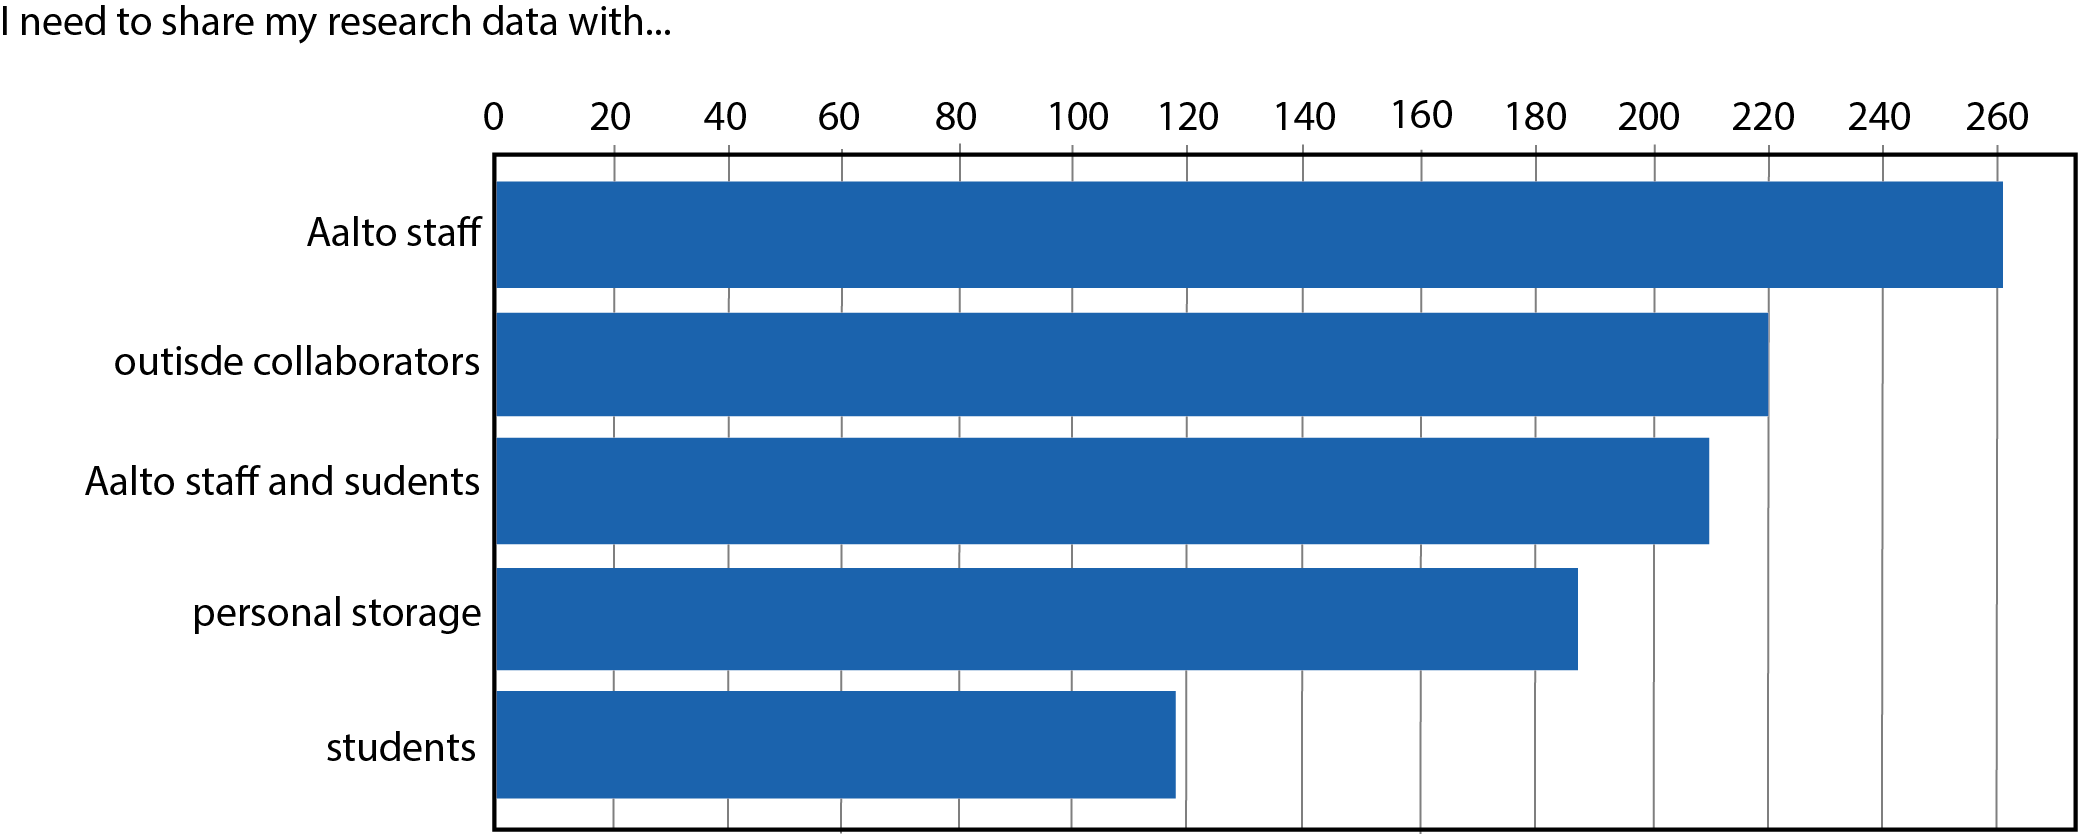
\includegraphics[width=\textwidth]{images/share_with}
    \end{centering}
    \caption{The different parties reserch data has to be shared with - horizontal axis is the amount of respondents}
    \label{fig:share_with}
\end{figure}

The types of files people would need to save are very varied - the most
popular type of files are Microsoft Office style files (text documents and
spreadsheets) and PDF files. Different image, video, sound, code and other
formats are brought up in the questionnaire, even virtual machine images.
The amount of required storage space varies from 10Gt to over 500Gt, as shown
in Figure \ref{fig:size}. The most
common storage time for research data is measured in years, since that
is the scope of research projects and data management is required throughout
the project. The distribution of required storage times is shown in Figure
\ref{fig:time}.


\begin{figure}
    \begin{centering}
        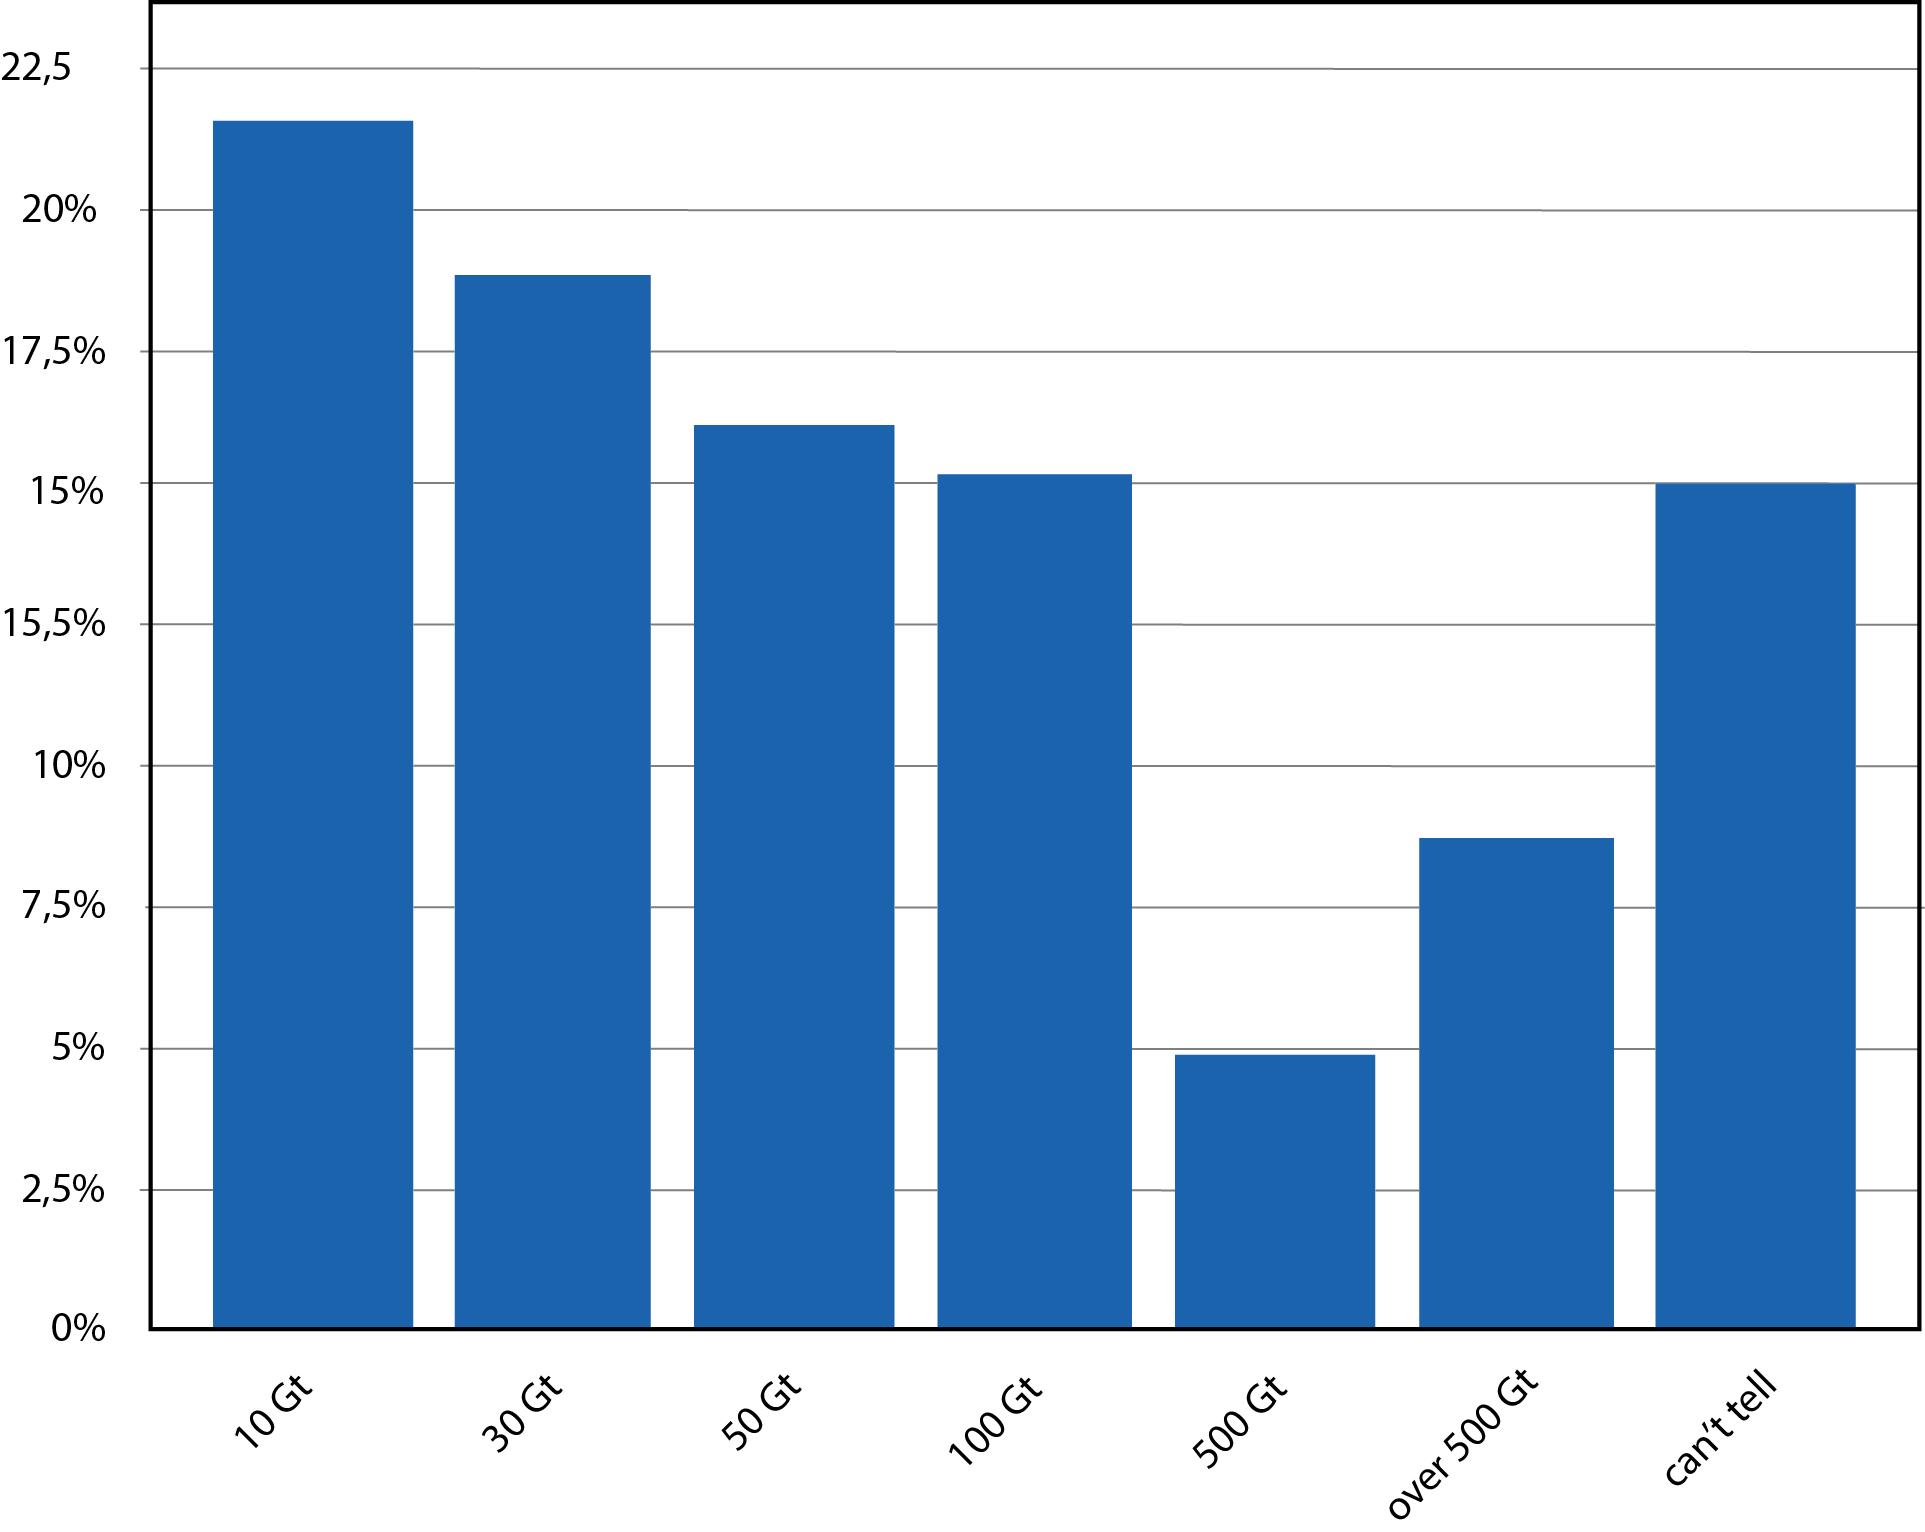
\includegraphics[width=\textwidth]{images/size}
    \end{centering}
    \caption{The required storage capacities according to the respondents - vertical
             axis is the percentage of respondents}
    \label{fig:size}
\end{figure}

\begin{figure}
    \begin{centering}
        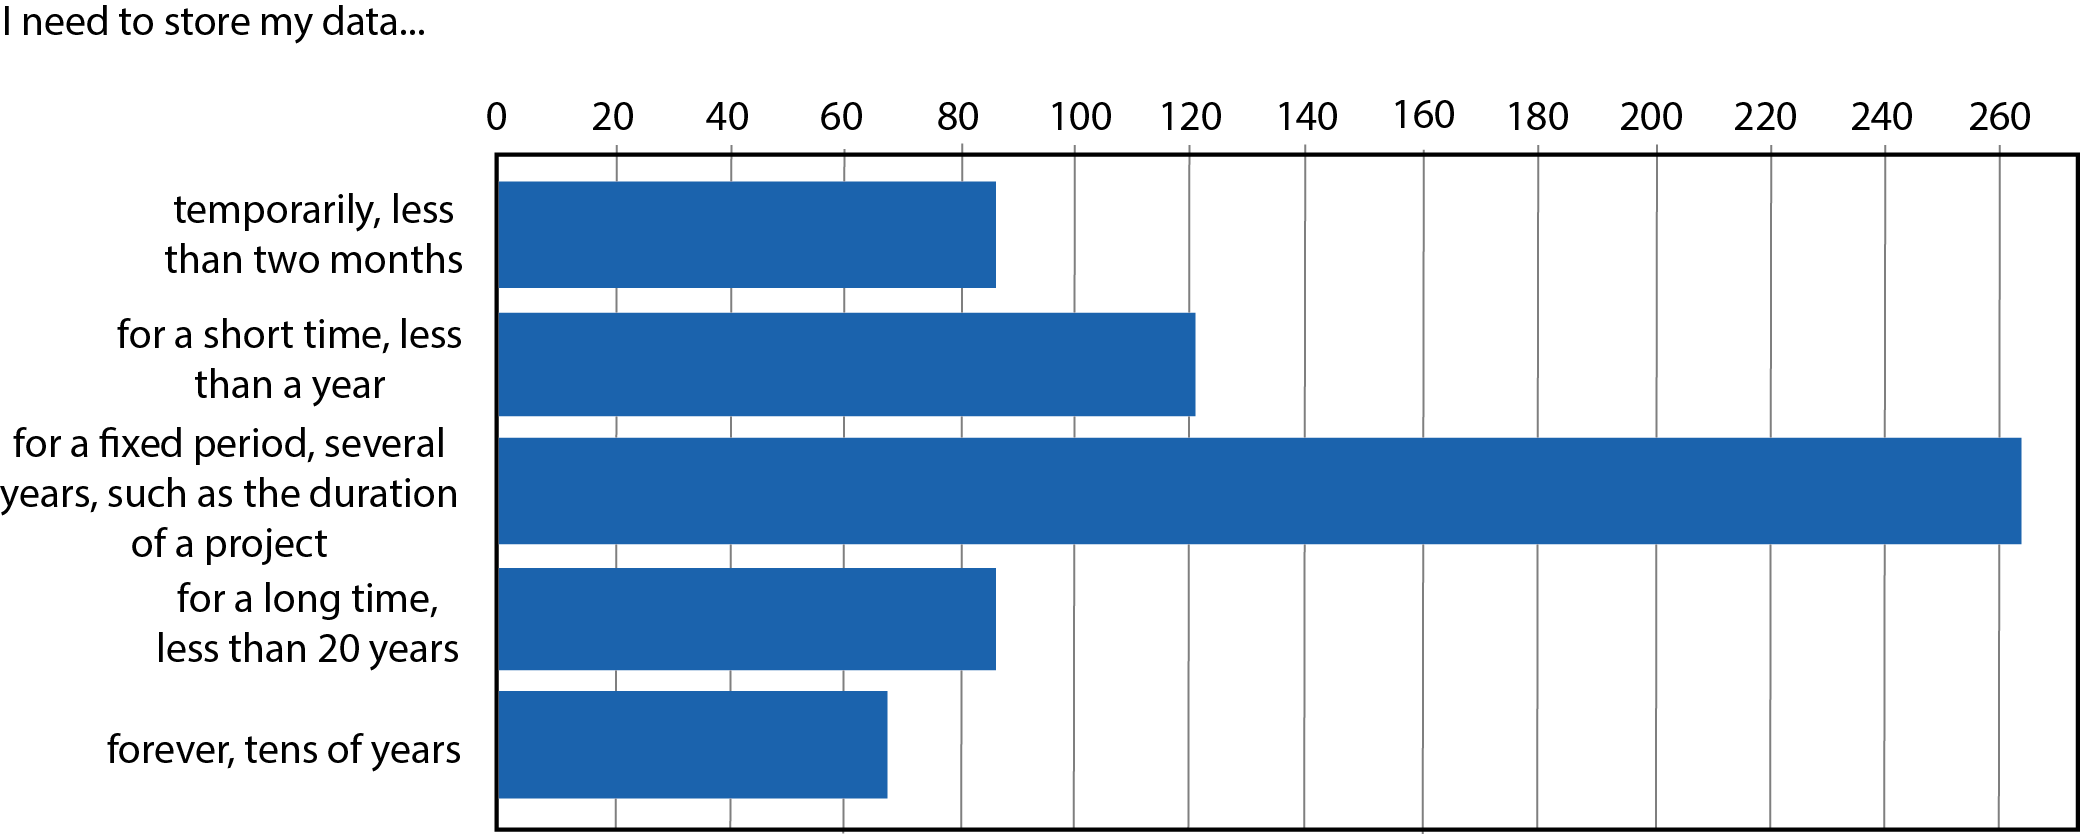
\includegraphics[width=\textwidth]{images/time}
    \end{centering}
    \caption{The required storage time of datasets - the horizontal axis is the amount
             of respondents}
    \label{fig:time}
\end{figure}

Most of the respondents of the second questionnaire handle their research data
every day and their research data is confidential. Not all confidential data
needs to be shared outside Aalto University, but most respondents had to do
that from time to time.

Most of the respondents use existing cloud services, such as Google Drive or
Dropbox to do research data management during their projects. The systems are
used both out of necessity (there is no existing Aalto infrastructure, for
example, to have non-Aalto people working on the same datasets or files) and
because they are easy to use and people have experience from using them from
outside of work. For some, this is not an option, since some data has to be
stored in Finland and the cloud providers cannot comply to that request.

These studies show that there are indeed a need already in place for a system to
manage and share research data in Aalto. In addition training and policies to support data
management through the lifecycle of data are required. Existing cloud based solutions, such
as Google Drive and Dropbox are the benchmark that people use to compare
existing and future solutions to. This sets a bar for the solutions that
would be implemented to address research data management and publication
challenges.

\section{Benchmarking existing solutions}
\label{sec:benchmarking}

Technical solutions to publishing and managing research data exist already, many
of them open source and free. Some of the solutions were mentioned in the
literature review in section \ref{sec:implementations_literature}. This section describes
those systems and some other in more practical detail. The benchmarking was
done using online demo versions of the software, reading the related
documentation and in some cases examining the source codes and installation
processes that they required.

For a more visual overview, see Section \ref{chapter:conclusions} for an
overview table of existing solutions. The Section \ref{chapter:prototype}
contains a more in depth look into the Dataverse system and the installation
processes of Hydra Project and Zenodo.

This is not a comprehensive listing of repository systems. Many institutions
have implemented their own systems and other, non-institute related systems
exist as well. The benchmark solutions presented here have been chosen due to
their wide adoption.

Harvard Dataverse is a Harvard University originated open source system
for research data publication. This system was benchmarked by both reading the
relevant documentation as well as making a local installation for testing
purposes - more on the test installation on Section \ref{chapter:prototype}.
It is implemented with Java and is available
online at GitHub\footnote{\url{https://github.com/IQSS/dataverse}}. Dataverse
uses Apache Solr\footnote{\url{http://lucene.apache.org/solr/}} to index its
PostgreSQL\footnote{\url{http://www.postgresql.org/}} database to facilitate
faceted search. For server software you can use Glassfish\footnote{\url{https://glassfish.java.net/}}
or Apache\footnote{\url{https://httpd.apache.org/}}.

Their website\footnote{\url{http://dataverse.org/}} reports that the Dataverse
software would be installed in 12 universities around the world. This
number does not include, for example, the Jyväskylä Universiy Dataverse which makes
it reasonable to assume that there are other Dataverses out in the world. The
main Harvard Dataverse\footnote{\url{https://dataverse.harvard.edu/}}, which
is the biggest Dataverse instance around, contains 59 652 datasets that contain
288 174 files as of writing this thesis.

Dataverse offers a wide range of features. It generates citeable DOIs for
datasets published in it and it also allows the administrator of the system
to use Handle identifiers\footnote{\url{https://www.handle.net/}} out of the
box as well. It has a publishing workflow that allows for saving of drafts and
review before publishing. Faceted metadata based fulltext search makes datasets
discoverable and metadata can be added both to the dataset level and the file
level. The access control system built into Dataverse allows permissions to be
granted to individuals and groups alike. The access controls can also be
integrated with Shibboleth\footnote{\url{https://shibboleth.net/}}, which is in
wide use across research institutions across the globe. For a full list of
features, source code and other relevant information see the links in the
footnotes.

Dataverse allows manual upload of datasets and an API to explore datasets
and upload them programmatically. Once published, new versions of datasets
can be uploaded and all the versions remain visible. Dataverse also includes the the
TwoRavens\footnote{\url{http://datascience.iq.harvard.edu/about-tworavens}} application
for visualizing tabular datasets.

Dataverse is a functional system for publishing research data. It is not a tool
for managing research data during the research project, but it could be used
even during that time to share research data with collaborators. It also does
not offer long term archival options.

CKAN\footnote{\url{http://ckan.org/}} is an open source data portal software that aims to make data available
over the Internet. CKAN instance was not installed for the purposes of this
thesis, but a demo CKAN cite\footnote{\url{http://demo.ckan.org/}} was tested
in addition to the documentation being read. CKAN is implemented in Python and
it uses Apache Solr to to index a PostgreSQL database, much like Dataverse.

CKAN offers full text search of dataset metadata and versioning of datasets.
CKAN also allows for robust customization and data visualization as well as
uploads through a web interface and an API. The access controls to the CKAN
are coarse grained, public sharing of datasets or sharing withing an
organization. CKAN is also promotes its extensibility, and indeed it has been
adopted, for example, as the frontend of the CSC's
services\footnote{\url{https://github.com/kata-csc}}. What separates CKAN from
the other repository solutions is that it offers extensive geospatial features.

CKAN is designed for publishing and sharing data and not for managing data
during the project it's being created.

Invenio\footnote{\url{http://invenio.readthedocs.org/en/latest/}} is a CERN
originated digital library management software. It started as the CERN
documentation server, hosting over 1 000 000 bibliographic records and is now
available at the public domain\footnote{\url{https://github.com/inveniosoftware}}.
Zenodo\footnote{\url{https://zenodo.org/}}
is a CERN run public instance of Invenio with a thin UI layer on top. The EUDAT
B2Share service\footnote{\url{https://b2share.eudat.eu/?ln=en}} also runs on
Invenio. Invenio installation was tried using the source code of Zenodo to get
a better grasp of the system.

Invenio is built with Python and it implements similar features as the other
systems discussed earlier in this section. Fulltext metadata search, uploads
through an API and web UI and other repository features are present. Zenodo is
integrated with GitHub and it gives the option to publish source code as a
citeable scientific entity. Invenio itself has the capability to implement
different persistent identifier methods - Zenodo has chosen to use DOI and
EUDAT B2Share used Handle out of the box.

Invenio is like Dataverse - a tool to publish digital assets but not
for managing data during research.

A side note from EUDAT is that they have also implemented a Dropbox-like
service called B2Drop\footnote{\url{https://eudat.eu/services/b2drop}},
which is targeted to researches that want to share
reseach data during the research project. EUDAT project source code for
both B2Share and B2Drop
is also available online\footnote{\url{https://github.com/EUDAT-B2SHARE},
\url{https://github.com/EUDAT-B2DROP}}.

The Hydra project is an open source digital repository solution. The Hydra
solution was also tested during the writing of this thesis by installing and
setting up the system in addition to reading the related documentation and
trying available instances.

The Hydra project is a Ruby on Rails\footnote{\url{http://rubyonrails.org/}}
application built on top of the Fedora repository software\footnote{\url{http://www.fedora-commons.org/}}.
It uses a project called Blacklight\footnote{\url{http://projectblacklight.org/}}
for the discovery platform and similarly to Dataverse it uses Apache Solr to
index data stored in the Fedora repository. The code for the Hydra project is
available at GitHub\footnote{\url{https://github.com/projecthydra}} and the
developer community maintains a wiki online\footnote{\url{https://wiki.duraspace.org/display/hydra/The+Hydra+Project}}. The Hydra website lists 29 universities and institutions that have
adopted the Hydra software, mostly in the USA.

Hydra project is very flexible - it is used around the world for institutional
repositories, museum websites, cultural heritage storage and other similar
projects. Extensibility comes with a price, since an out of the box Hydra
installation requires the user to configure all the types of data you would
need for your chosen repository. Many implementations do exist, since Hydra
has been adopted around the world, but despite the fact that these solutions
are open source they are still tightly connected to the institutions that
implemented them, demanding still work if they were to be adopted to a new
institution. Some Hydra versions have dataset versioning implemented.

Hydra project is aimed to archiving and publishing data. It is not designed as
a tool for managing data during research projects.

Aalto University has adopted Elsevier
Pure\footnote{\url{https://www.elsevier.com/solutions/pure}} as a tool for
researchers to manage their publications. The system allows for linking
datasets to your profile, but the version that is running at Aalto University
as of writing of this thesis does not support actually uploading datasets
to a repository. This brings up an integration point for future development,
since it would make sense that when you upload your datasets to a repository
it should show up in your researcher profile.

iRODS\footnote{\url{http://irods.org/}} is a data management software used by many research institutions to
manage research data. It is open source and available on GitHub\footnote{\url{https://github.com/irods}}
along with the many libraries and software components that come with it. iRODS
virtualizes storage hardware, which in part constitutes to the amount of
different software packages that go into it, since different hardware requires
different drivers and many contributors have implemented their own packages for
iRODS. For the purposes of this thesis an instance of iRODS was not installed,
but experts and users of the system were interviewed and documentation was read
along with the code.

In addition to virtualizing the storage hardware iRODS offers data discovery
by compiling metadata about the files and folders in the system to a metadata
catalog. The iRODS rules engine allows the users to program workflows and
automated events to the system. Newer versions (since iRODS 3) of iRODS allow
iRODS systems to be federated, which means that two iRODS systems from
different origins can share data easily.

iRODS is implemented in C++ and it offers client APIs for multiple programming
languages. iRODS also scales from single personal computers into large data
grids.

In Finland iRODS is in use at least in the University of Jyväskylä and in the
systems of CSC (the IDA system mentioned in Section \ref{sec:csc} uses iRODS).
The iRODS systems in Finland focus on enabling researcher collaboration, which
is the role iRODS is primarily designed for. The iRODS architecture is not
designed for sharing data, but could be used as a part of a system that shared
data.

GitHub\footnote{\url{https://github.com/}} has been mentioned a few times as
the place where the source code of many of the projects mentioned here resides.
It is a close analogue to sharing research data, since it is a platform to share
formatted information between collaborators and anyone who might be interested
in the source code. Being a widely adopted platform it also contains, for
example, lists to datasets\footnote{\url{https://github.com/caesar0301/awesome-public-datasets}}
available around the globe as well as datastreams\footnote{\url{https://github.com/HazeWatchApp}}
that you could use as a basis of applications serving greater public and good.
The Zenodo connection also makes source code citeable.

GitHub hosts, according to their own statistics as of writing of this thesis,
30.1 million code repositories. While the main appeal of GitHub is to allow
software to be written collaboratively (GitHub could be seen as the
collaborative extension to Git\footnote{\url{https://git-scm.com/}}), the
version control software. GitHub also hosts some data and visualizes that data.
What really sets GitHub apart from the research data sharing platforms is the
social aspects it contains. GitHub has powerful issue tracking systems,
commenting capabilities and it promotes good coding style and contribution
by rewarding the contributors with recognition.

GitHub is a Ruby on Rails application with Git and the required C daemons
integrated to it. Git makes it also tool for managing code during the research
project, making GitHub a solution for the entire lifetime of source code. There
is also GitLab\footnote{\url{https://about.gitlab.com/}}, that enables
institutions to set up their own GitHub-like systems.

\clearpage

\section{Solutions in Finland}
\label{sec:finland_current}

In Sections \ref{sec:expert_interviews} - \ref{sec:csc} the current situation
in Finland was touched from different perspectives. The Table \ref{table:finland} below summarizes
the learnings from different actors in Finland as well as some additional
findings. This list is not comprehensive but does contain the biggest
institutions. It's is liuely that other institutions and the institutions listed
below are working on more matters. All Finnish universities maintain a digital
publishing archive for papers and theses published in those universities - they
are not listed below. The footnotes are on the next page.

\captionof{table}{Actors in Finland and their actions as of writing of this thesis}
\label{table:finland}
\begin{tabularx}{\textwidth}{| >{\raggedright}p{3cm} | X |}
  \hline
  \textbf{Actor}                            & \textbf{Work currently underway} \\
  \hline
  \rowcolor{Gray}
  Ministry of Education and Culture         & The Open Science and Research Initiative\footnotemark,
                                              which entails services for publishing research data and metadata (mentioned
                                              before in Section \ref{sec:csc}). They also
                                              organize training to facilitate open research and research data in Finnish
                                              institutions. The Initiative also runs the Tuuli project, that aims to
                                              help researchers to make data management plans that are required nowadays
                                              by funding bodies.\\
  \hline
  CSC                                       & As the national provider of scientific computing services CSC works with
                                              all the major Finnish institutions. It is also the implementing force in
                                              many of the Ministry level projects. CSC is also the the Finnish contact
                                              point to EUDAT, the European Union level research data services.\\
  \hline
  \rowcolor{Gray}
  University of Helsinki                    & University of Helsinki has formulated its data policy\footnotemark~and
                                              is working towards implementing the infrastructure required to support
                                              it.\footnotemark\\
  \hline
  University of Jyväskylä                   & Unviersity of Jyväskylä has an own Dataverse instance and they are using
                                              iRODS as their research data management tool. They are also developing a
                                              desktop interface for iRODS to enable researcher collaboration.\\
  \hline
  \rowcolor{Gray}
  University of Tampere                     & University of Tampere operates the Finnish Social Science Data
                                              Archive\footnotemark, an resource center funded by the Ministry of
                                              Culture and Education to store datasets from the field of social
                                              science.\\
  \hline
  National Library of Finland               & The National Library manages the URN identifier scheme that can be
                                              used to get persistent identifiers to datasets and other scientific
                                              material in Finland. It's also involved in the long term storage
                                              project (PAS). It also runs Finna\footnotemark, a digital archive for
                                              Finnish museums, archives and libraries.\\
  \hline
  \rowcolor{Gray}
  Aalto University                          & Aalto University is forming its research data policy. \\
  \hline
\end{tabularx}

% Hack to get the footnotes correct from the table previous
\addtocounter{footnote}{-4}
\footnotetext{\url{http://openscience.fi/frontpage}}
\addtocounter{footnote}{1}
\footnotetext{\url{https://www.helsinki.fi/sites/default/files/atoms/files/datapolicy\_final\_en.pdf}} 
\addtocounter{footnote}{1}
\footnotetext{M. Nurmela and V. Tenhunen, personal communication, November 9th, 2015}
\addtocounter{footnote}{1}
\footnotetext{\url{http://www.fsd.uta.fi/en/index.html}}
\addtocounter{footnote}{1}
\footnotetext{\url{https://www.finna.fi/}}

\iffalse
Here we are going to paraphrase research and interesting things going on in
Finland at the moment. Items to look into would be:

\begin{itemize}
    \item IDA and Etsin services by CSC
    \item the ATT initiative going on
    \item the social science library by Tampere University
    \item the long term storage developed by national library
    \item national library also develops the URN schemes
\end{itemize}

A question to ask Keijo later is that many of the people interviewed told about
their upcoming research. Is it interesting here or should we stick to things
that exist for sure?
\fi

\section{Outcomes of the positioning research}
\label{sec:positioning_outcomes}

It is clear that research data management and publishing is not just a
technical problem. Perfectly fine technical solutions for publishing, sharing
and managing research data exist. However, a system
that would integrate these and make the whole lifecycle of research data -
from creation to archiving - does not exist. The challenge
of managing, sharing and publishing research data brings together experts from
multiple fields (researchers themselves, support staff in librarians and
science IT and the managers who oversee these transaction to name a few) and
this collaboration has not been figured out yet. Without proper technical
solutions there definitely can not be proper research data management, but
policies and culture have to be developed as well. There is little culture or reward to
going through the trouble of properly managing and publishing research data.

It also seems that the problem should not be solved independently by all the
institutions in Finland, let alone in the world. Successful research data
publishing solutions are open source software projects, that offer the base
solution for free and the institutions can then become part of the developer
community simultaneously improving the software and adapting it to their own
needs. Similarly iRODS, the tool for managing research data, is open source. In
addition to using similar tools as their peers different institutions should
consider also forming their policies and research data management guidelines
to be compatible. After all, one goal of sharing and publishing research data
is to make collaboration easier and make science better.

The insights gained from this positioning research and the learnings from
the literature review in Section \ref{chapter:background} and the next Section
\ref{chapter:prototype} will be discussed together in Sections
\ref{chapter:discussion} and \ref{chapter:conclusions}.

\iffalse
First of all, it is clear that the research data management is not jut a
technical problem. Perfectly fine technical solutions to the problems of
publishing research data and managing your data in a safe way exist but the
real problem is to get people and organizations to use them.

Research data management questions transcend the university level as well
as the national borders. After all, the goal of publishing and sharing
research data is to make science move forward in a faster clip and make the
quality of research better by collaboration - ergo there is no point in every
institution in Finland to manage their own research data repositories and
archives.

With this in mind this thesis focuses on providing a prototype solution that
serves as a wireframe for implementation that should be done in such a way that
all institutions in Finland would benefit from that. In addition this research
will provide a road map style solution that would make use of existing know-how
and work and serve as a possible proposal on how to bring research data
management into all Finnish institutions that need that kind of service.
\fi
